\documentclass[
    paper=a4,
    % fontsize=12,
    % DIV=calc,
    parskip=half,
% ]{scrreprt}
]{scrartcl}


\usepackage[T1]{fontenc}	
\usepackage[utf8]{inputenc}
\usepackage[ngerman]{babel}
\usepackage{microtype}
\usepackage{libertine}
\usepackage[libertine]{newtxmath} 

\usepackage[dvipsnames]{xcolor}
\usepackage{booktabs}
\usepackage{graphicx}
\usepackage{subcaption}
\usepackage{pdfpages}
\usepackage{svg}
\usepackage[
    locale		=	DE, 					%	Deutsche Normen
	detect-all,								%	Richtige Font im Textmodus/Mathemodus
	per-mode	=	fraction,				%	Bruchstrich darstellen
	range-units	=	repeat,					%	Einheiten wiederholt darstellen bei sirange
	range-phrase=	{{ bis }},	
]{siunitx}
\usepackage{amsmath}
\usepackage{circuitikz}

\RequirePackage{listingsutf8}					% add source code

\usepackage{hyperref}

\renewcommand*{\familydefault}{\sfdefault}


\definecolor{colordarkblue}{HTML}{4C1DCC}			% color for internal links
\definecolor{colorblue}{HTML}{0480CC}				% color for weblinks
\definecolor{colorgreen}{HTML}{26CC1B}				% color for citations
\definecolor{coloryellow}{HTML}{F0B707}				% color for missing macro
\definecolor{colorred}{HTML}{CC1204}				% color for edit macro
\colorlet{colorgray}{black!40}						% color for editedit macro


\KOMAoptions{
    numbers=noendperiod,
}

\hypersetup{
    bookmarksnumbered   =   true,
    breaklinks          =   true,
    colorlinks          =   true,
    linkcolor           =   colordarkblue,
    urlcolor            =   colorblue,
    citecolor           =   colorgreen,
    pdftitle            =   {Labor 8 Jan Hoegen},
    pdfsubject          =   {Versuchsvorbereitung Labor Digitaltechnik},    
    pdfauthor           =   {Von Jan Hoegen},
}

\ctikzset{
    logic ports=european,
    logic ports/scale=1.0,
    logic ports/fill=lightgray,
    tripoles/european not symbol=ieee circle,
}
\usetikzlibrary{babel}

\newcommand{\tikzmark}[1]{\tikz[overlay,remember picture] \node (#1) {};}
\newcommand{\DrawBox}[3][]{%
    \tikz[overlay,remember picture]{
    \draw[black,#1]
      ($(#2)+(-0.5em,2.0ex)$) rectangle
      ($(#3)+(0.75em,-0.75ex)$);}
}

\lstset{%
	frame			=	tb ,							%	hline top and bottom
	breaklines		=	true,							%	break lines
	rulecolor		=	\color{black} ,					%	linecolor black
	keywordstyle	=	\color{blue} ,
	commentstyle	=	\color{ForestGreen} ,
	stringstyle		=	\color{Mulberry} ,
	title			=	\lstname ,						%	set filename as title 
	basicstyle		=	\footnotesize\ttfamily ,		%	set font
	numbers			=	left,							%	numbers left
	xleftmargin		=	2em,							%	set length on left side
	framexleftmargin=	1em,
	inputencoding	=	utf8,  							% Input encoding
    extendedchars	=	true,  							% Extended ASCII
}
\lstdefinestyle{TeX}{language=TeX,						%	more keyword for TeX
    morekeywords={vspace, hspace, rule, ifdefined, newcommand, setlength, newlength, RequirePackage, ProvidesPackage, NeedsTeXFormat, DeclareOption, ProcessOption, usepackage, documentclass, authorone, authortwo, authorthree, begin, thanks, reversemarginpar, ProcessOptions, definecolor, small, sffamily, AtBeginDocument, newenvironment, cbcolor, textcolor, emph, renewcommand}, 
}
\lstset{literate=										%	T1 in listing
  {á}{{\'a}}1 {é}{{\'e}}1 {í}{{\'i}}1 {ó}{{\'o}}1 {ú}{{\'u}}1
  {Á}{{\'A}}1 {É}{{\'E}}1 {Í}{{\'I}}1 {Ó}{{\'O}}1 {Ú}{{\'U}}1
  {à}{{\`a}}1 {è}{{\`e}}1 {ì}{{\`i}}1 {ò}{{\`o}}1 {ù}{{\`u}}1
  {À}{{\`A}}1 {È}{{\'E}}1 {Ì}{{\`I}}1 {Ò}{{\`O}}1 {Ù}{{\`U}}1
  {ä}{{\"a}}1 {ë}{{\"e}}1 {ï}{{\"i}}1 {ö}{{\"o}}1 {ü}{{\"u}}1
  {Ä}{{\"A}}1 {Ë}{{\"E}}1 {Ï}{{\"I}}1 {Ö}{{\"O}}1 {Ü}{{\"U}}1
  {â}{{\^a}}1 {ê}{{\^e}}1 {î}{{\^i}}1 {ô}{{\^o}}1 {û}{{\^u}}1
  {Â}{{\^A}}1 {Ê}{{\^E}}1 {Î}{{\^I}}1 {Ô}{{\^O}}1 {Û}{{\^U}}1
  {ã}{{\~a}}1 {ẽ}{{\~e}}1 {ĩ}{{\~i}}1 {õ}{{\~o}}1 {ũ}{{\~u}}1
  {Ã}{{\~A}}1 {Ẽ}{{\~E}}1 {Ĩ}{{\~I}}1 {Õ}{{\~O}}1 {Ũ}{{\~U}}1
  {œ}{{\oe}}1 {Œ}{{\OE}}1 {æ}{{\ae}}1 {Æ}{{\AE}}1 {ß}{{\ss}}1
  {ű}{{\H{u}}}1 {Ű}{{\H{U}}}1 {ő}{{\H{o}}}1 {Ő}{{\H{O}}}1
  {ç}{{\c c}}1 {Ç}{{\c C}}1 {ø}{{\o}}1 {å}{{\r a}}1 {Å}{{\r A}}1
  {€}{{\euro}}1 {£}{{\pounds}}1 {«}{{\guillemotleft}}1
  {»}{{\guillemotright}}1 {ñ}{{\~n}}1 {Ñ}{{\~N}}1 {¿}{{?`}}1 {¡}{{!`}}1 
  {~}{{\textasciitilde}}1 {*}{{\normalfont{*}}}1
}

\graphicspath{/Anhang}

\newcommand{\shadowsection}[1]{%
	\refstepcounter{section}
	\addcontentsline{toc}{section}{\protect\numberline{\thesection}{#1}}
}

\newcommand{\legend}[1]{\par\footnotesize\textbf{Legende}: #1\par}
\newcommand{\figsource}[1]{\par\footnotesize\textbf{Quelle:} #1\par}

\newcommand{\quoteenv}[1]{\glqq #1\grqq} 

\newcommand{\edit}[1]{\textcolor{colorred}{#1}}

\newcommand{\missing}{%
    \textcolor{coloryellow}{MISSING}%
	\PackageWarning{\jobname}{You used the 'missing' macro at this line. Remove it before finalising document.}%
}


\titlehead{
    \textsc{Hochschule Karlsruhe}\\
    University of Applied Sciences\\
    Fakultät für Elektro- und Informationstechnik
    % Studiengang EITB SS 22
    }
\subject{Studiengang Elektro- und Informationstechnik (Bachelor)}
\title{Versuchsvorbereitung Labor Digitaltechnik}
\subtitle{Versuch 8: Das letzte Gefecht}
\author{%
    Jan Hoegen%
    \thanks{Matrikelnumer: 82358. E-Mail: \href{mailto:hoja1028@h-ka.de}{hoja1028@h-ka.de}.}
}
\publishers{Betreuer: Prof. Dr.\,-Ing. Jan Bauer}
\date{Erstellt am \today}


\begin{document}

\maketitle

\tableofcontents

\newpage

\section{Analyse des Systementwurfs}

    \subsection{Erklärung des Top-Level-Systementwurfs}
        Es werden die einzelnen Schaltblöcke des Top-Level-Systementwurfs erklärt.

        \begin{description}
            \item[input\_synchronizer] Stellt sicher, dass das Eingangssignal der Lichtschranken zwischen \SI{0}{\volt} und $V_{cc}$ liegt.
            \item[statemachine] Das Signal der Lichtschranken wird analysiert und der aktuelle Zustand bestimmt. Daraufhin werden Zählrichtung und Zählimpuls an die Speicherblöcke \textit{decade\_counter} weitergeleitet.
            \item[decade\_counter] Hier werden der Wert der Einerstelle und der Zehnerstelle getrennt gespeichert. Erhält die Einerstelle einen Impuls von der \textit{statemachine}, so wird um den Wert 1 hoch- bzw runtergezählt.   Die Richtung wird durch das Signal \textit{dir} bestimmt. Die Zehnerstelle wird durch ein Overflow- bzw. Underflowsignal der Einerstelle angesteuert.
            \item[sevenseg\_decoder] Schließlich wird der aktuelle Wert der Speicher decodiert, sodass die 7-Segment-Anzeige die zugehörige Dezimalziffer anzeigt.
        \end{description}

    \subsection{Zählrichtung definieren}
        Wenn das Signal \textit{dir} auf 1 gesetzt ist, wird vorwärts gezählt und um 1 inkrementiert. Bei $dir=0$ wird abwärts gezählt.

    \subsection{Ein- und Ausfahrt detektieren durch Lichtschranken}
        Signalverlauf \textit{opt\_switch}: S2 S1.
        
        \begin{tabular}{cc}\toprule
            Einfahrt    &   Ausfahrt\\\midrule
            00          &   00\\
            01          &   10\\
            11          &   11\\
            10          &   01\\
            00          &   00\\\bottomrule
        \end{tabular}

    \subsection{Ansteuerung der Einerstelle des Dekadenzählers}
        Der Dekadenzähler zählt immer dann in die vorgegebene Richtung, wenn eine positive Taktflanke anliegt und der Eingang \textit{enable} auf 1 gesetzt ist. 
        
        Solange also $enable=0$ gilt, wird der aktuelle Zustand beibehalten. Genau dann, wenn \textit{statemachine} feststellt, dass das Aus- bzw. Einfahren beendet ist, wird \textit{enable} für eine Periode auf 1 gesetzt. Der Speicher zählt somit um einen Wert weiter.
        
    \subsection{Ansteuerung der Zehnerstelle des Dekadenzählers}
        Wenn für die Einerstelle ein Overflow von 9 auf 0 oder ein Underflow von 0 auf 9 erfolgt, wird das Signal \textit{ripple} des COUNTER\_LOW für eine Periode auf 1 gesetzt. Dieses Signal wird an den \textit{enable}-Eingang des COUNTER\_HIGH angeschlossen. Dieser zählt also in genau diesem Fall um einen Wert weiter. 

    \subsection{Beschriftung der Top-Level-Signale}
        Abbildung \ref{fig:1} zeigt die Beschriftung der Top-Level-Signale.

    \begin{figure}[hb]
        \centering
        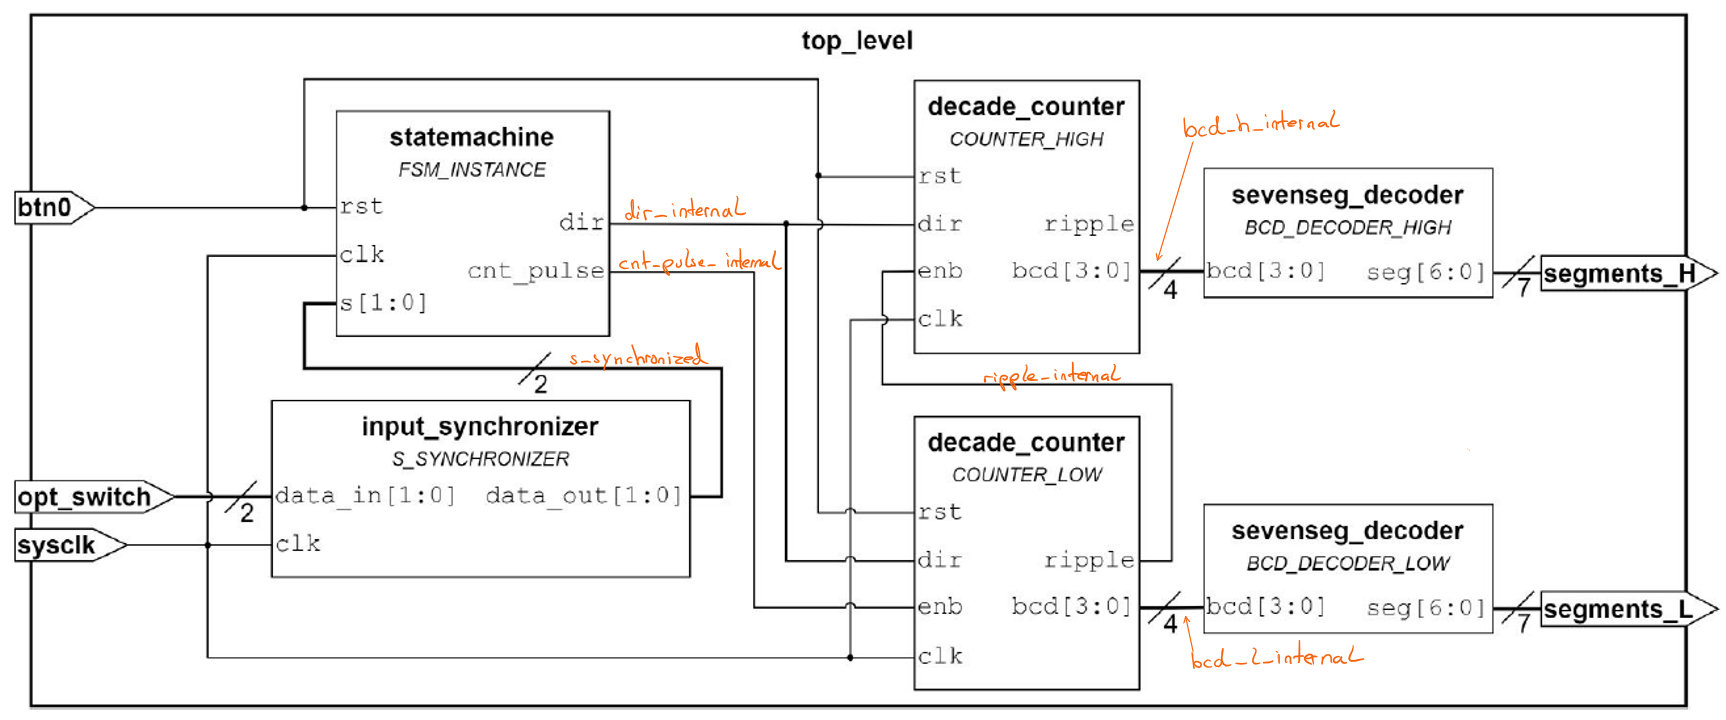
\includegraphics[width=0.9\textwidth]{top_level.png}
        \caption{Beschriftung der Top-Level-Signale}
        \label{fig:1}
    \end{figure}

\section{Verständnis des Automaten}

    \subsection{Moore oder Mealy?}
        Da der Ausgang vom aktuellen Zustand un dem Eingang abhängt, liegt ein Mealy-Automat vor. 

    \subsection{Vervollständigen der Simulation}
        Da S2 das MSB ist, muss Simulation 1 zu Szenario B gehören und Simulation 2 zu Szenario A. Abbildung \ref{fig:2} zeigt die vervollständigte Simulation.

        \begin{figure}[hb]
            \centering
            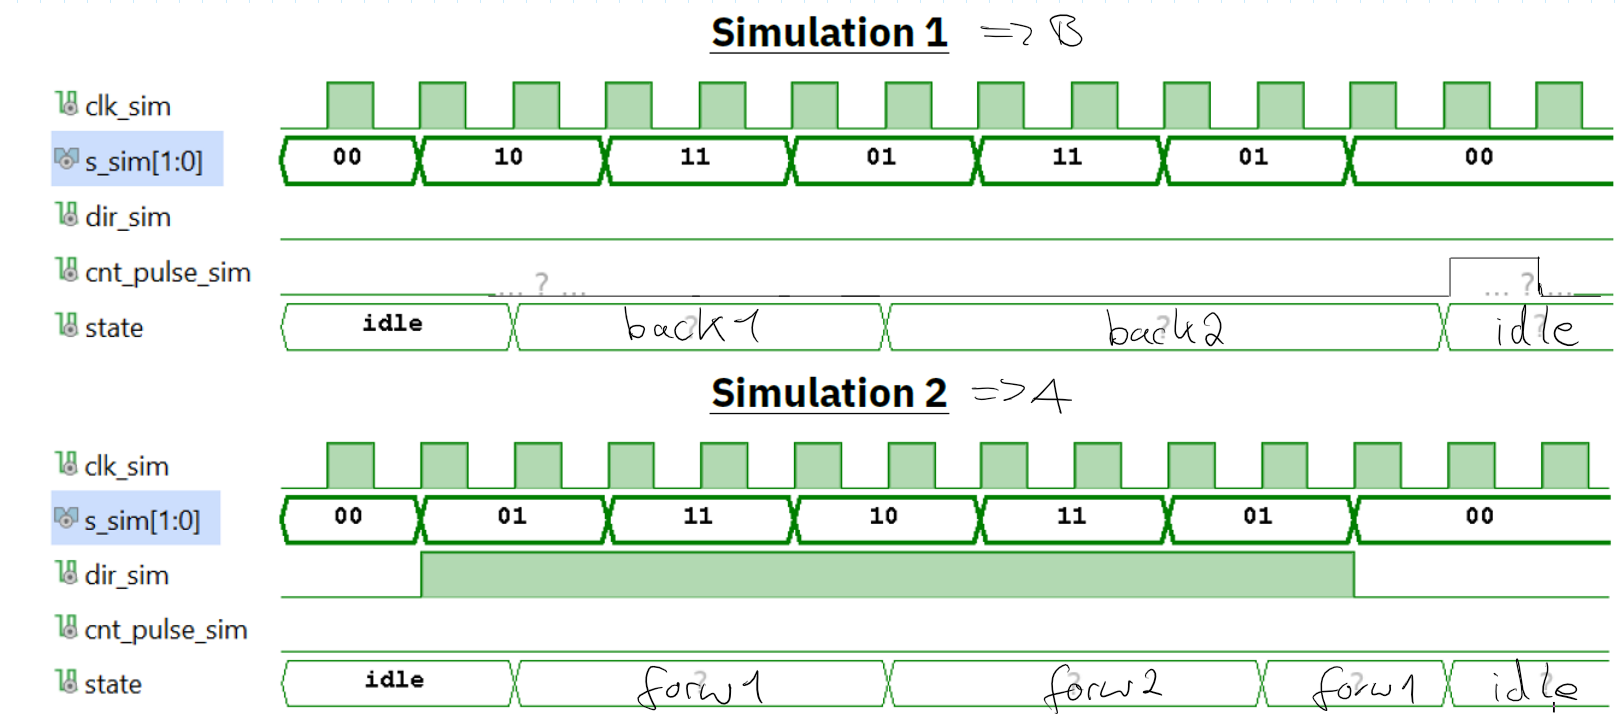
\includegraphics[width=0.8\textwidth]{simulation.png}  
            \caption{Vervollständigen der Simulation}
            \label{fig:2}
        \end{figure}

\section{Auswahl der I/O-Pins}
    Abbildung \ref{fig:3} zeigt die Pinbelegung des FPGA.

    \begin{figure}[hb]
        \centering
        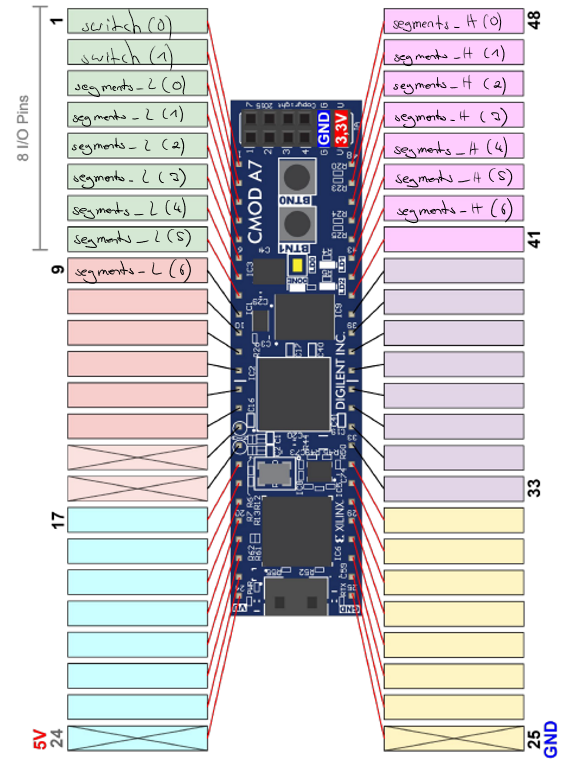
\includegraphics[width=0.5\textwidth]{pinbelegung.png}  
        \caption{Pinbelegung des FPGA}
        \label{fig:3}
    \end{figure}

\section{Wissen transferieren}

    \subsection{Verständnis der Anlasswiederholsperre}
        Die Zustände werden als Variablentyp in VHDL definiert. Damit lassen sie sich auf leicht verständliche Weise referenzieren und in case-Statements verwenden.

        Indem zwei Prozesse verwendet, werden, lassen sich Speicher und Kombinatorik getrennt voneinander betrachten. Im kombinatorischen Teil werden durch ÜSN und ASN festgelegt, welchen Wert der nächste Zustand haben wird. Im sequentiellen Prozess wird festgelegt, wann der Zustandswechsel erfolgt.
        
        In einem case-Statement können die Zustände, die vorher als Variablentypen definiert wurden, als einzelne Fälle betrachtet werden. Durch If-Anweisungen werden die Eingangssignale überprüft und der entspreche Output gesetzt. Außerdem wird damit der nächste Zustand festgelegt.

        warum case gtu geeignet?

        wie werden übergange realisiert?
        wie viele verzweigungen gibt es

    \subsection{Transformation auf den Mealy-Automanten}

        wie viele when fälle

        wie viele if zweige für jeden zustand

\end{document}
